% Options for packages loaded elsewhere
\PassOptionsToPackage{unicode}{hyperref}
\PassOptionsToPackage{hyphens}{url}
%
\documentclass[
  ignorenonframetext,
]{beamer}
\usepackage{pgfpages}
\setbeamertemplate{caption}[numbered]
\setbeamertemplate{caption label separator}{: }
\setbeamercolor{caption name}{fg=normal text.fg}
\beamertemplatenavigationsymbolsempty
% Prevent slide breaks in the middle of a paragraph
\widowpenalties 1 10000
\raggedbottom
\setbeamertemplate{part page}{
  \centering
  \begin{beamercolorbox}[sep=16pt,center]{part title}
    \usebeamerfont{part title}\insertpart\par
  \end{beamercolorbox}
}
\setbeamertemplate{section page}{
  \centering
  \begin{beamercolorbox}[sep=12pt,center]{part title}
    \usebeamerfont{section title}\insertsection\par
  \end{beamercolorbox}
}
\setbeamertemplate{subsection page}{
  \centering
  \begin{beamercolorbox}[sep=8pt,center]{part title}
    \usebeamerfont{subsection title}\insertsubsection\par
  \end{beamercolorbox}
}
\AtBeginPart{
  \frame{\partpage}
}
\AtBeginSection{
  \ifbibliography
  \else
    \frame{\sectionpage}
  \fi
}
\AtBeginSubsection{
  \frame{\subsectionpage}
}
\usepackage{lmodern}
\usepackage{amssymb,amsmath}
\usepackage{ifxetex,ifluatex}
\ifnum 0\ifxetex 1\fi\ifluatex 1\fi=0 % if pdftex
  \usepackage[T1]{fontenc}
  \usepackage[utf8]{inputenc}
  \usepackage{textcomp} % provide euro and other symbols
\else % if luatex or xetex
  \usepackage{unicode-math}
  \defaultfontfeatures{Scale=MatchLowercase}
  \defaultfontfeatures[\rmfamily]{Ligatures=TeX,Scale=1}
\fi
% Use upquote if available, for straight quotes in verbatim environments
\IfFileExists{upquote.sty}{\usepackage{upquote}}{}
\IfFileExists{microtype.sty}{% use microtype if available
  \usepackage[]{microtype}
  \UseMicrotypeSet[protrusion]{basicmath} % disable protrusion for tt fonts
}{}
\makeatletter
\@ifundefined{KOMAClassName}{% if non-KOMA class
  \IfFileExists{parskip.sty}{%
    \usepackage{parskip}
  }{% else
    \setlength{\parindent}{0pt}
    \setlength{\parskip}{6pt plus 2pt minus 1pt}}
}{% if KOMA class
  \KOMAoptions{parskip=half}}
\makeatother
\usepackage{xcolor}
\IfFileExists{xurl.sty}{\usepackage{xurl}}{} % add URL line breaks if available
\IfFileExists{bookmark.sty}{\usepackage{bookmark}}{\usepackage{hyperref}}
\hypersetup{
  pdftitle={Part C: Visualizing COVID-19},
  pdfauthor={Alisa Ishikawa},
  hidelinks,
  pdfcreator={LaTeX via pandoc}}
\urlstyle{same} % disable monospaced font for URLs
\newif\ifbibliography
\usepackage{color}
\usepackage{fancyvrb}
\newcommand{\VerbBar}{|}
\newcommand{\VERB}{\Verb[commandchars=\\\{\}]}
\DefineVerbatimEnvironment{Highlighting}{Verbatim}{commandchars=\\\{\}}
% Add ',fontsize=\small' for more characters per line
\usepackage{framed}
\definecolor{shadecolor}{RGB}{248,248,248}
\newenvironment{Shaded}{\begin{snugshade}}{\end{snugshade}}
\newcommand{\AlertTok}[1]{\textcolor[rgb]{0.94,0.16,0.16}{#1}}
\newcommand{\AnnotationTok}[1]{\textcolor[rgb]{0.56,0.35,0.01}{\textbf{\textit{#1}}}}
\newcommand{\AttributeTok}[1]{\textcolor[rgb]{0.77,0.63,0.00}{#1}}
\newcommand{\BaseNTok}[1]{\textcolor[rgb]{0.00,0.00,0.81}{#1}}
\newcommand{\BuiltInTok}[1]{#1}
\newcommand{\CharTok}[1]{\textcolor[rgb]{0.31,0.60,0.02}{#1}}
\newcommand{\CommentTok}[1]{\textcolor[rgb]{0.56,0.35,0.01}{\textit{#1}}}
\newcommand{\CommentVarTok}[1]{\textcolor[rgb]{0.56,0.35,0.01}{\textbf{\textit{#1}}}}
\newcommand{\ConstantTok}[1]{\textcolor[rgb]{0.00,0.00,0.00}{#1}}
\newcommand{\ControlFlowTok}[1]{\textcolor[rgb]{0.13,0.29,0.53}{\textbf{#1}}}
\newcommand{\DataTypeTok}[1]{\textcolor[rgb]{0.13,0.29,0.53}{#1}}
\newcommand{\DecValTok}[1]{\textcolor[rgb]{0.00,0.00,0.81}{#1}}
\newcommand{\DocumentationTok}[1]{\textcolor[rgb]{0.56,0.35,0.01}{\textbf{\textit{#1}}}}
\newcommand{\ErrorTok}[1]{\textcolor[rgb]{0.64,0.00,0.00}{\textbf{#1}}}
\newcommand{\ExtensionTok}[1]{#1}
\newcommand{\FloatTok}[1]{\textcolor[rgb]{0.00,0.00,0.81}{#1}}
\newcommand{\FunctionTok}[1]{\textcolor[rgb]{0.00,0.00,0.00}{#1}}
\newcommand{\ImportTok}[1]{#1}
\newcommand{\InformationTok}[1]{\textcolor[rgb]{0.56,0.35,0.01}{\textbf{\textit{#1}}}}
\newcommand{\KeywordTok}[1]{\textcolor[rgb]{0.13,0.29,0.53}{\textbf{#1}}}
\newcommand{\NormalTok}[1]{#1}
\newcommand{\OperatorTok}[1]{\textcolor[rgb]{0.81,0.36,0.00}{\textbf{#1}}}
\newcommand{\OtherTok}[1]{\textcolor[rgb]{0.56,0.35,0.01}{#1}}
\newcommand{\PreprocessorTok}[1]{\textcolor[rgb]{0.56,0.35,0.01}{\textit{#1}}}
\newcommand{\RegionMarkerTok}[1]{#1}
\newcommand{\SpecialCharTok}[1]{\textcolor[rgb]{0.00,0.00,0.00}{#1}}
\newcommand{\SpecialStringTok}[1]{\textcolor[rgb]{0.31,0.60,0.02}{#1}}
\newcommand{\StringTok}[1]{\textcolor[rgb]{0.31,0.60,0.02}{#1}}
\newcommand{\VariableTok}[1]{\textcolor[rgb]{0.00,0.00,0.00}{#1}}
\newcommand{\VerbatimStringTok}[1]{\textcolor[rgb]{0.31,0.60,0.02}{#1}}
\newcommand{\WarningTok}[1]{\textcolor[rgb]{0.56,0.35,0.01}{\textbf{\textit{#1}}}}
\usepackage{graphicx,grffile}
\makeatletter
\def\maxwidth{\ifdim\Gin@nat@width>\linewidth\linewidth\else\Gin@nat@width\fi}
\def\maxheight{\ifdim\Gin@nat@height>\textheight\textheight\else\Gin@nat@height\fi}
\makeatother
% Scale images if necessary, so that they will not overflow the page
% margins by default, and it is still possible to overwrite the defaults
% using explicit options in \includegraphics[width, height, ...]{}
\setkeys{Gin}{width=\maxwidth,height=\maxheight,keepaspectratio}
% Set default figure placement to htbp
\makeatletter
\def\fps@figure{htbp}
\makeatother
\setlength{\emergencystretch}{3em} % prevent overfull lines
\providecommand{\tightlist}{%
  \setlength{\itemsep}{0pt}\setlength{\parskip}{0pt}}
\setcounter{secnumdepth}{-\maxdimen} % remove section numbering

\title{Part C: Visualizing COVID-19}
\author{Alisa Ishikawa}
\date{January 5, 2020}

\begin{document}
\frame{\titlepage}

\begin{frame}{Generic Plot() Function}
\protect\hypertarget{generic-plot-function}{}

\begin{itemize}
\tightlist
\item
  Basic function in R
\item
  2D format
\item
  Correlation
\item
  Scatter plots and line graphs
\end{itemize}

The generic syntax for the Plot function is:

\textbf{Plot(x,y\ldots)}

\end{frame}

\begin{frame}{Advanced Plot() Function}
\protect\hypertarget{advanced-plot-function}{}

Advanced Plot function syntax is:

\begin{quote}
\textbf{plot(x, y, type, main, sub, xlab, ylab)}
\end{quote}

where\ldots{}

``\textbf{p}'': points\\
``\textbf{l}'': lines\\
``\textbf{b}'': both point and lines in a single place\\
``\textbf{c}'': join empty point by the lines\\
``\textbf{o}'': both lines and over-plotted point\\
``\textbf{h}'': histogram ``\textbf{s}'': stair steps\\
``\textbf{n}'': no plotting

``\textbf{xlab}'': x-axis legends\\
``\textbf{ylab}'': y-axis legends

\end{frame}

\begin{frame}{Example Exercise}
\protect\hypertarget{example-exercise}{}

Exam grades of 10 students in two courses, X and Y, respectively\\

\begin{quote}
X = 40, 15, 50, 12, 22, 29, 21, 35, 14, 15\\
Y = 41, 42, 32, 14, 42, 27, 13, 50, 33, 22
\end{quote}

\end{frame}

\begin{frame}[fragile]{Exercise 1: Define X and plot as lines plot}
\protect\hypertarget{exercise-1-define-x-and-plot-as-lines-plot}{}

\begin{Shaded}
\begin{Highlighting}[]
\NormalTok{X =}\StringTok{ }\KeywordTok{c}\NormalTok{(}\DecValTok{40}\NormalTok{, }\DecValTok{15}\NormalTok{, }\DecValTok{50}\NormalTok{, }\DecValTok{12}\NormalTok{, }\DecValTok{22}\NormalTok{, }\DecValTok{29}\NormalTok{, }\DecValTok{21}\NormalTok{, }\DecValTok{35}\NormalTok{, }\DecValTok{14}\NormalTok{, }\DecValTok{15}\NormalTok{)}
\KeywordTok{plot}\NormalTok{(X ,}\DataTypeTok{type =} \StringTok{"l"}\NormalTok{)}
\end{Highlighting}
\end{Shaded}

\includegraphics[width=0.8\linewidth]{Visualizing-COVID-19-using-R_files/figure-beamer/plot-1}

\end{frame}

\begin{frame}[fragile]{Exercise 2: Define Y and plot as points plot}
\protect\hypertarget{exercise-2-define-y-and-plot-as-points-plot}{}

\begin{Shaded}
\begin{Highlighting}[]
\NormalTok{Y =}\StringTok{ }\KeywordTok{c}\NormalTok{(}\DecValTok{41}\NormalTok{, }\DecValTok{42}\NormalTok{, }\DecValTok{32}\NormalTok{, }\DecValTok{14}\NormalTok{, }\DecValTok{42}\NormalTok{, }\DecValTok{27}\NormalTok{, }\DecValTok{13}\NormalTok{, }\DecValTok{50}\NormalTok{, }\DecValTok{33}\NormalTok{, }\DecValTok{22}\NormalTok{)}
\KeywordTok{plot}\NormalTok{(Y ,}\DataTypeTok{type =} \StringTok{"p"}\NormalTok{)}
\end{Highlighting}
\end{Shaded}

\includegraphics[width=0.8\linewidth]{Visualizing-COVID-19-using-R_files/figure-beamer/plot2-1}

\end{frame}

\begin{frame}{Plot() Function Capabilities}
\protect\hypertarget{plot-function-capabilities}{}

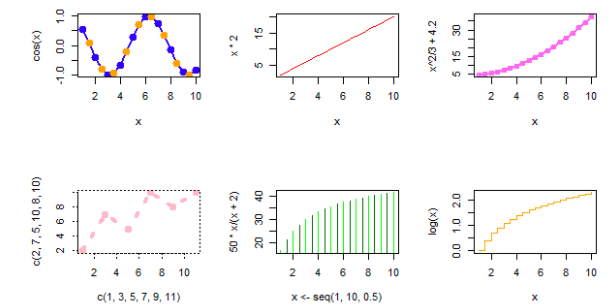
\includegraphics[width=1\textwidth,height=\textheight]{/Users/alisaishikawa/Downloads/Data Science/HSF-MIBM2-COVID19/Images/plot function other examples.png}

\end{frame}

\begin{frame}[fragile]{Alternative Visulization Tools: ggplots()}
\protect\hypertarget{alternative-visulization-tools-ggplots}{}

\begin{verbatim}
install.packages("ggplot2")
\end{verbatim}

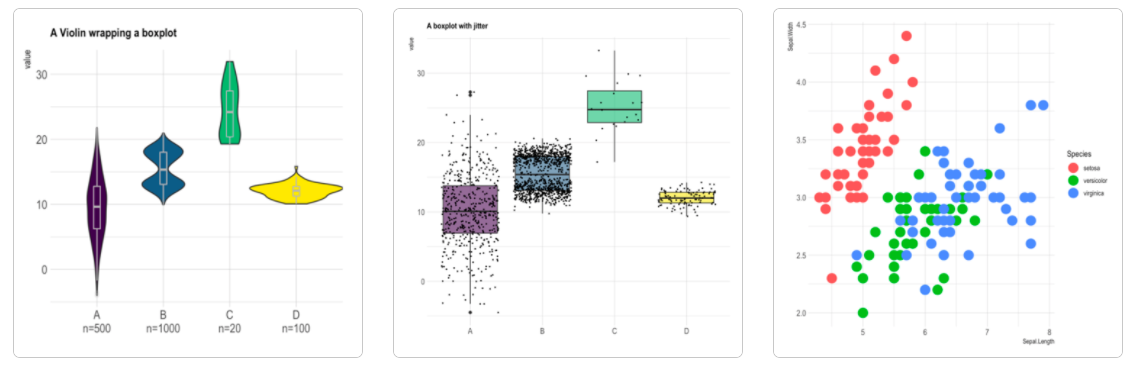
\includegraphics[width=0.65\textwidth,height=\textheight]{/Users/alisaishikawa/Downloads/Data Science/HSF-MIBM2-COVID19/Images/ggplot other 1.png}\\
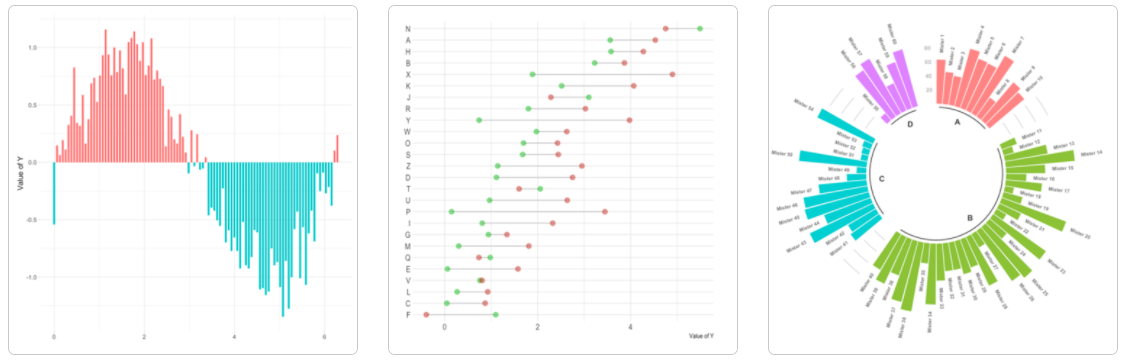
\includegraphics[width=0.65\textwidth,height=\textheight]{/Users/alisaishikawa/Downloads/Data Science/HSF-MIBM2-COVID19/Images/ggplot other 2.png}\\
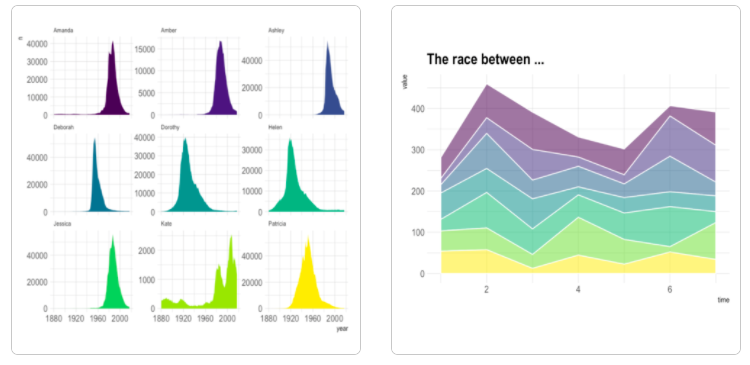
\includegraphics[width=0.5\textwidth,height=\textheight]{/Users/alisaishikawa/Downloads/Data Science/HSF-MIBM2-COVID19/Images/ggplot other 3.png}

\end{frame}

\begin{frame}[fragile]{Case Study: Visualization of COVID-19}
\protect\hypertarget{case-study-visualization-of-covid-19}{}

Package: nCov2019\\
By: Dr.~Guangchuang Yu (Southern Medical University)

\begin{verbatim}
remotes::install_github("GuangchuangYu/nCov2019")  
\end{verbatim}

\begin{block}{Explore 1st Impression of dataset}

Assign x and y

\begin{verbatim}
x <- get_nCov2019()
y <- load_nCov2019()
\end{verbatim}

Check results for x and y

\begin{verbatim}
x
  
China (total confirmed cases): 95901
last update: 2020-12-21 20:45:32
\end{verbatim}

\begin{verbatim}
y
  
nCov2019 historical data 
last update: 2020-11-26 
\end{verbatim}

\end{block}

\end{frame}

\begin{frame}[fragile]{Summary of worldwide data}
\protect\hypertarget{summary-of-worldwide-data}{}

\begin{verbatim}
x['global']
\end{verbatim}

\begin{verbatim}
    name           confirm   suspect dead    deadRate  showRate  heal
1   China          95901      7      4771    4.97      FALSE     89480
2   United States  18277433   0      324898  1.78      FALSE     10622096
3   India          10055560   0      145810  1.45      FALSE     9606111
4   Brazil         7238600    0      186764  2.58      FALSE     6409986
5   Russia         2850042    0      50723   1.78      FALSE     2273510
6   France         2529756    0      60665   2.4       FALSE     189638
7   United Kingdom 2079564    0      67718   3.26      FALSE     4380
8   Turkey         2043704    0      18351   0.9       FALSE     1834705
9   Italy          1964054    0      69214   3.52      FALSE     1281258
10  Spain          1817448    0      48926   2.69      FALSE     196958
11  Argentina      1541285    0      41813   2.71      FALSE     1368346
12  Germany         1531998   0      26655   1.74      FALSE     1129280
\end{verbatim}

\end{frame}

\begin{frame}{Visualize with line graph using ggplot()}
\protect\hypertarget{visualize-with-line-graph-using-ggplot}{}

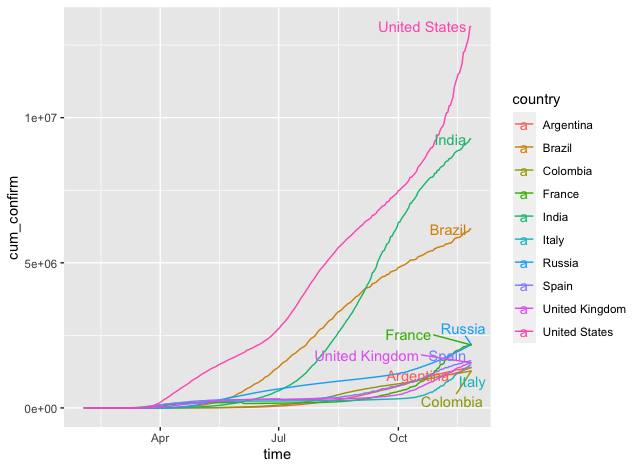
\includegraphics[width=0.8\textwidth,height=\textheight]{/Users/alisaishikawa/Downloads/Data Science/HSF-MIBM2-COVID19/Images/Top 10 graph.png}

\end{frame}

\begin{frame}[fragile]{Visualize a static map with plot()}
\protect\hypertarget{visualize-a-static-map-with-plot}{}

\begin{verbatim}
install.packages("maps")  
\end{verbatim}

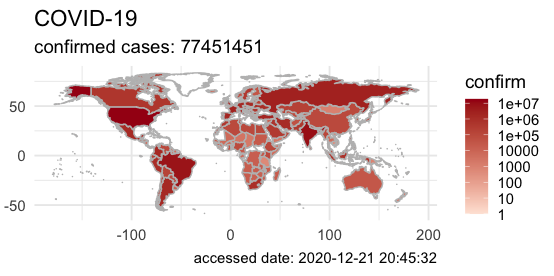
\includegraphics[width=1\textwidth,height=\textheight]{/Users/alisaishikawa/Downloads/Data Science/HSF-MIBM2-COVID19/Images/Static Map 21.12.png}

\end{frame}

\begin{frame}[fragile]{Visualize a moving map with magick()}
\protect\hypertarget{visualize-a-moving-map-with-magick}{}

\begin{verbatim}
install.packages("magick")  
\end{verbatim}

\includegraphics[width=1\textwidth,height=\textheight]{/Users/alisaishikawa/Downloads/Data Science/HSF-MIBM2-COVID19/Images/moving map.gif}

\end{frame}

\end{document}
